% Figure 4 — decision-value waterfall (standalone, auto-cropped vector PDF).
% Compile: pdflatex figure4_waterfall.tex  ->  figure4_waterfall.pdf
\documentclass[border=2pt]{standalone}
\usepackage{mathptmx}
\usepackage{amsmath,amssymb}
\usepackage{tikz}
\usepackage{pgfplots}
\pgfplotsset{compat=1.17}
\begin{document}
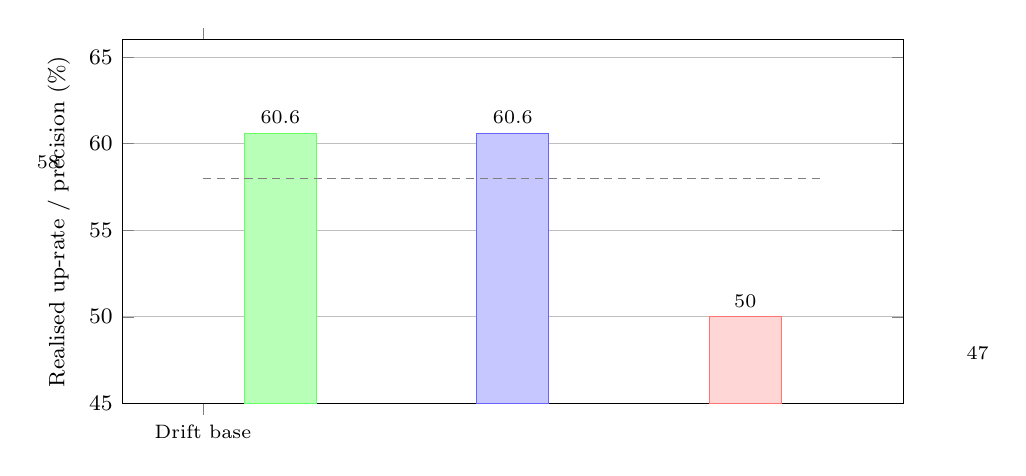
\begin{tikzpicture}
\begin{axis}[
  width=11.5cm, height=6.2cm, font=\footnotesize,
  ybar, bar width=26pt,
  symbolic x coords={Drift base,Selection,Fired prec.,Ranking acc.,AUC read.},
  xtick=data, x tick label style={font=\scriptsize},
  ymin=45, ymax=66, ylabel={Realised up-rate / precision (\%)},
  enlarge x limits=0.13, ymajorgrids,
  nodes near coords, every node near coord/.append style={font=\scriptsize},
]
\addplot[fill=gray!25,draw=gray!60] coordinates {(Drift base,58.0)};
\addplot[fill=green!28,draw=green!60] coordinates {(Selection,60.6)};
\addplot[fill=blue!22,draw=blue!60] coordinates {(Fired prec.,60.6)};
\addplot[fill=red!16,draw=red!55] coordinates {(Ranking acc.,50.0)};
\addplot[fill=red!10,draw=red!45] coordinates {(AUC read.,47.0)};
\draw[densely dashed,gray] (axis cs:Drift base,58.0) -- (axis cs:AUC read.,58.0);
\end{axis}
\end{tikzpicture}
\end{document}
